\documentclass{report}
\usepackage[utf8]{inputenc}
\usepackage{amsmath}
\usepackage{amsfonts}
\usepackage{hyperref}
\usepackage{tcolorbox}
\usepackage{breqn}
\usepackage{adjustbox}
\usepackage{changepage}
\usepackage{rotating}
\usepackage{algorithm}
\usepackage{algpseudocode}
\usepackage{ntheorem}
\usepackage[table,xcdraw]{xcolor}
\usepackage{longtable}

% Definition
\newtheorem{definition}{Definition}{\bfseries}{\itshape}
\newtheorem*{definition*}{Definition}{\bfseries}{\itshape}

% Theorem
\newtheorem{theorem}{Theorem}{\bfseries}{\itshape}

% Concept
\newtheorem*{concept}{}{\bfseries}{\itshape}

\title{Comparing AES and DES}
\author{Ana Clara Zoppi Serpa\\ Prof. Dr. Ricardo Dahab \\ Dr. Jorge Nakahara Jr.}
\date{\today}

\begin{document}

\maketitle

\tableofcontents

\chapter{Comparing AES and DES}
In this chapter, we provide a comparison of two classical ciphers, AES \cite{AES-FIPS} and \cite{DES-FIPS}. They are both NIST standards, with AES being the chosen to replace DES. We compare them with respect to their general structure, their diffusion process, their $S$-Boxes and their vulnerability against DC \cite{ShamirBook}, LC \cite{Matsui1993LinearCM} and exhaustive key search \cite{DESCracker} attacks. We assume the reader is familiar with:
\begin{itemize}
    \item The AES cipher structure, available in \textcolor{red}{Chapter X}
    \item The DES cipher structure, available in \textcolor{red}{Chapter X}
    \item Block cipher, Feistel Network and Substitution Permutation Network definitions, available in \textcolor{red}{Chapter X}
    \item The ANF analysis conducted in \textcolor{red}{Chapter X}
    \item The diffusion analysis of DES conducted in \textcolor{red}{Chapter X}
    \item The diffusion analysis of AES conducted in \textcolor{red}{Chapter X}
    \item The Differential Cryptanalysis overview conducted in \textcolor{red}{Chapter X}
    \item The Linear Cryptanalysis overview conducted in \textcolor{red}{Chapter X}
\end{itemize}

%\section{Notation}

\section{Acronyms}
\begin{itemize}
    \item AES: Advanced Encryption Standard
    \item DES: Data Encryption Standard
    \item NIST: National Institute of Standards and Technology
    \item $S$-Box: Substitution Box
    \item ANF: Algebraic Normal Form
    \item DC: Differential Cryptanalysis
    \item LC: Linear Cryptanalysis
    \item LAT: Linear Approximation Table
    \item DDT: Differential Distribution Table
\end{itemize}

\section{Comparative chart}

From \textcolor{red}{Chapters X, Y and Z}, we know the general structures of AES and DES, the fact that they are both iterated block ciphers, AES being an SPN and DES being a Feistel Network. We also know their parameter sets (block size, key size), their most common state representations, how many rounds are required in order to achieve complete plaintext and key diffusion, the ANFs of their $S$-Boxes, and their differential and linear uniformities. These pieces of information allow us to devise Table \ref{tbl:aes-vs-des}, which compares the two ciphers.

\begin{longtable}[c]{|ccc|}
\hline
\multicolumn{1}{|c|}{\textbf{Cipher}}                                & \multicolumn{1}{c|}{\textbf{AES}}               & \textbf{DES}             \\ \hline
\endfirsthead
%
\endhead
%
\multicolumn{1}{|c|}{\textbf{Reference}}                             & \multicolumn{1}{c|}{\cite{AES-FIPS}}                          & \cite{DES-FIPS}                        \\ \hline
\multicolumn{1}{|c|}{\textbf{Standardization process}}               & \multicolumn{1}{c|}{open contest}               & secret design            \\ \hline
\multicolumn{1}{|c|}{\textbf{Standardization time}}                  & \multicolumn{1}{c|}{2001}                       & 1977                     \\ \hline
\multicolumn{1}{|c|}{\textbf{Environment}}                           & \multicolumn{1}{c|}{hardware and software}      & hardware                 \\ \hline
\multicolumn{3}{|c|}{\textbf{General structure}}                                                                                                  \\ \hline
\multicolumn{1}{|c|}{\textbf{Type}}                                  & \multicolumn{1}{c|}{SPN}                        & Feistel Network          \\ \hline
\multicolumn{1}{|c|}{\textbf{Iterated}}                              & \multicolumn{1}{c|}{yes}                        & yes                      \\ \hline
\multicolumn{1}{|c|}{\textbf{Block size (bits)}}                     & \multicolumn{1}{c|}{128}                        & 64                       \\ \hline
\multicolumn{1}{|c|}{\textbf{Key size(s) (bits)}}                    & \multicolumn{1}{c|}{128, 192, 256}              & 64                       \\ \hline
\multicolumn{1}{|c|}{\textbf{Number of rounds}}                      & \multicolumn{1}{c|}{10, 12, 14}                 & 16                       \\ \hline
\multicolumn{1}{|c|}{\textbf{State representation}}                  & \multicolumn{1}{c|}{$4\times4$ matrix of bytes} & 1-dimensional bit vector \\ \hline
\multicolumn{1}{|c|}{\textbf{Basic data unit}}                       & \multicolumn{1}{c|}{byte}                       & bit                      \\ \hline
\multicolumn{1}{|c|}{\textbf{Key schedule}}                          & \multicolumn{1}{c|}{nonlinear}                  & linear                   \\ \hline
\multicolumn{1}{|c|}{\textbf{Algebraic structure}}                   & \multicolumn{1}{c|}{GF($2^8$) (polynomials)}    & GF(2) (bits only)        \\ \hline
\multicolumn{3}{|c|}{\textbf{Diffusion}}                                                                                                          \\ \hline
\multicolumn{1}{|c|}{\textbf{Rounds until full plaintext diffusion}} & \multicolumn{1}{c|}{2}                          & 5                        \\ \hline
\multicolumn{1}{|c|}{\textbf{Rounds until full key diffusion}}       & \multicolumn{1}{c|}{2, 3, 3}                    & 5                        \\ \hline
\multicolumn{1}{|c|}{\textbf{Diffusion components}}                  & \multicolumn{1}{c|}{\shortstack{\\ \texttt{ShiftRows}, \texttt{MixColumns}, \\ $S$-Boxes (bit level)}}      & $P$, $S$-Boxes               \\ \hline
\multicolumn{1}{|c|}{\textbf{MDS matrix usage}}                      & \multicolumn{1}{c|}{yes}                        & no                       \\ \hline
\multicolumn{3}{|c|}{\textbf{$S$-Boxes}}                                                                                                          \\ \hline
\multicolumn{1}{|c|}{\textbf{Quantity}}                              & \multicolumn{1}{c|}{1}                          & 8                        \\ \hline
\multicolumn{1}{|c|}{\textbf{Invertible}}                            & \multicolumn{1}{c|}{yes}                        & no                       \\ \hline
\multicolumn{1}{|c|}{\textbf{Input size(s)}}                         & \multicolumn{1}{c|}{8}                          & 6                        \\ \hline
\multicolumn{1}{|c|}{\textbf{Output size(s)}}                        & \multicolumn{1}{c|}{8}                          & 4                        \\ \hline
\multicolumn{1}{|c|}{\textbf{ANF(s) degree(s)}}                      & \multicolumn{1}{c|}{7}                          & 5                        \\ \hline
\multicolumn{1}{|c|}{\textbf{Differential uniformity}}               & \multicolumn{1}{c|}{4}                          & 16                       \\ \hline
\multicolumn{1}{|c|}{\textbf{Linear uniformity}}                     & \multicolumn{1}{c|}{16}                         & 14, 16, 18, 20           \\ \hline
\multicolumn{3}{|c|}{\textbf{Attacks}}                                                                                                            \\ \hline
\multicolumn{1}{|c|}{\textbf{Differential Cryptanalysis}}            & \multicolumn{1}{c|}{resistant}                  & vulnerable               \\ \hline
\multicolumn{1}{|c|}{\textbf{Linear Cryptanalysis}}                  & \multicolumn{1}{c|}{resistant}                  & vulnerable               \\ \hline
\multicolumn{1}{|c|}{\textbf{Exhaustive key search}}                 & \multicolumn{1}{c|}{resistant}                  & vulnerable               \\ \hline
\caption{Comparing AES and DES}
\label{tbl:aes-vs-des}
\end{longtable}

\section{Remarks}
With respect to the DC attack, it is worth noting that the DES design attempted at thwarting it by sharing plaintext bits between different $S$-Boxes by means of the extension function $E$, as outlined by \cite{Coppersmith1994}. That led Biham and Shamir \cite{ShamirBook} to seek alternatives to successfully attack DES other than the exploitation of the high differential uniformity of the $S$-Boxes. In order to successfully attack DES, they carefully constructed characteristics with maximum probability along the cipher's iterations, activating $3$ $S$-Boxes ($S_1, S_2$ and $S_3$) simultaneously with a characteristic of probability approximately equal to $1/234$. The fact that plaintext bits are shared between adjacent $S$-Boxes whilst key bits are not lead us to the need of computing joint DDTs for thorough analysis of the DES $S$-Boxes, i.e we need the joint DDTs to find non-zero entries which could be useful when constructing characteristics for DC attacks. However, with respect to LC, Matsui \cite{Matsui1993LinearCM} is able to exploit the high linear uniformity (equal to 20) of the $S_5$ $S$-Box of DES to mount a successful LC attack.

In the case of AES, both attacks (DC and LC) were taken into account (\cite{Susan}, \cite{Rijndael} and \cite{WideTrail2001} provide further detail on this). The diffusion process in AES, through the usage of the MDS matrix, ensures that \emph{the number of active $S$-Boxes increases exponentially along the cipher iterations}. Consequently, the probability of a characteristic (in the case of DC) and the bias of a linear relation (in the case of LC) decrease drastically. These small probabilities increase the required amount of plaintexts (chosen, for DC, and known, for LC) for the attacks, rendering DC and LC infeasible --- the required amount of plaintexts surpasses the size of the AES codebook. In DES, however, the diffusion through the $P$ permutation does not ensure a sufficient increase in the number of active $S$-Boxes, thus it is possible to find characteristics (and linear relations) with suitable probability, requiring an amount of plaintexts that does not surpass DES's codebook, and therefore making the attacks feasible (although computationally expensive).

In conclusion, the diffusion process of AES is able to thwart DC and LC attacks, whilst the diffusion process of DES is not, and the usage of an MDS matrix in the \texttt{MixColumns} transformation plays a central role in that (see Section \ref{sec:mc-and-diffusion}). Tables \ref{tbl:aes-dc} and \ref{tbl:aes-lc} outline AES's resistance against DC and LC, respectively. Since the AES block size is 128 bits, its codebook comprises all possible values of 128 bits, thus $2^{128}$ elements. In Tables \ref{tbl:aes-dc} and \ref{tbl:aes-lc}, it is possible to see that, at iteration 4, the amount of required plaintexts surpasses $2^{128}$ (and therefore DC and LC attacks cannot be mounted).

% Please add the following required packages to your document preamble:
% \usepackage{longtable}
% Note: It may be necessary to compile the document several times to get a multi-page table to line up properly
\begin{longtable}[c]{|c|c|c|c|c|}
\hline
\textbf{Iterations} & \textbf{\begin{tabular}[c]{@{}c@{}}Minimum\\ number of \\ active $S$-Boxes\end{tabular}} & \textbf{\begin{tabular}[c]{@{}c@{}}Total\\ of active\\ $S$-Boxes\end{tabular}} & \textbf{\begin{tabular}[c]{@{}c@{}}Probability\\ of a characteristic\end{tabular}} & \textbf{\begin{tabular}[c]{@{}c@{}}Required\\ chosen\\ plaintexts\end{tabular}} \\ \hline
\endfirsthead
%
\endhead
%
1                   & $1$                                                                                      & $1$                                                                            & $\leq 2^{-6}$                                                                      & $2^6$                                                                           \\ \hline
2                   & $4^1 = 4$                                                                                & $5$                                                                            & $\leq (2^{-6})^5 = 2^{-30}$                                                        & $2^{30}$                                                                          \\ \hline
3                   & $4^2 = 16$                                                                               & $21$                                                                           & $\leq (2^{-6})^{21} = 2^{-126}$                                                      & $2^{126}$                                                                         \\ \hline
4                   & $\geq 4$                                                                                 & $\geq 25$                                                                      & $\leq (2^{-6})^{25} = 2^{-150}$                                                      & $2^{150}$                                                                         \\ \hline
\caption{AES's resistance against DC}
\label{tbl:aes-dc}
\end{longtable}

The differential uniformity (see \textcolor{red}{Chapter X}) of the AES $S$-Box is 4, and the total of possible entries of its DDT is $2^8 = 256$. Therefore, if one AES $S$-Box is active, the maximum probability of a characteristic is $4/256 = 2^{-6}$. If 5 $S$-Boxes are active, the maximum probability is $(2^{-6})^5$, and so forth. The required amount of chosen plaintexts is approximately the inverse of the probability, and thus, on iteration $4$, since more than 25 $S$-Boxes will be active, a DC attack becomes infeasible (the amount of required plaintexts surpasses the codebook).

% Please add the following required packages to your document preamble:
% \usepackage{longtable}
% Note: It may be necessary to compile the document several times to get a multi-page table to line up properly
\begin{longtable}[c]{|c|c|c|c|c|}
\hline
\textbf{Iterations} & \textbf{\begin{tabular}[c]{@{}c@{}}Mininum\\ number of\\ active $S$-Boxes\end{tabular}} & \textbf{\begin{tabular}[c]{@{}c@{}}Total \\ of active\\ $S$-Boxes\end{tabular}} & \textbf{\begin{tabular}[c]{@{}c@{}}Bias\\ of a linear relation\end{tabular}} & \textbf{\begin{tabular}[c]{@{}c@{}}Required\\ known\\ plaintexts\end{tabular}} \\ \hline
\endfirsthead
%
\endhead
%
1                   & $1$                                                                                     & $1$                                                                             & $\leq (2^{-4})^1 \times 2^0 = 2^{-4}$                                                     & $2^8$                                                                          \\ \hline
2                   & $4^1 = 4$                                                                               & $5$                                                                             & $\leq (2^{-4})^5\times2^4 = 2^{-16}$                                                & $2^{32}$                                                                       \\ \hline
3                   & $4^2 = 16$                                                                              & $21$                                                                            & $\leq (2^{-4})^{21}\times2^{20} = 2^{-64}$                                          & $2^{128}$                                                                      \\ \hline
4                   & $\geq 4$                                                                                & $\geq 25$                                                                       & $\leq (2^{-4})^{25}\times2^{24} = 2^{-76}$                                          & $2^{152}$                                                                      \\ \hline
\caption{AES's resistance against LC}
\label{tbl:aes-lc}
\end{longtable}

For LC, similar analysis applies. The linear uniformity of the AES $S$-Box is 16, and the total of possible entries of its LAT is $2^8 = 256$. The bias of a random variable (linear relation) $X_{i_1} \oplus X_{i_2} \oplus ... \oplus X_{i_k}$ is $\epsilon_{i_1, i_2, ..., i_k} = 2^{k-1} \prod_{j=1}^{k} \epsilon_{i_j}$ (see \textcolor{red}{Chapter X}). In the case of a single active $S$-Box, $k = 1$, therefore the bias of a linear relation is $2^{-4}$. For 4 active $S$-Boxes, the maximum bias is $(2^{-4})^5\times2^4 = 2^{-16}$, and so forth. The necessary known plaintexts are approximately $1/\epsilon^2$, where $\epsilon$ is the bias, therefore an LC attack becomes infeasible at iteration 4.

\subsection{\texttt{MixColumns} and the number of active $S$-Boxes throughout the AES iterations}\label{sec:mc-and-diffusion}

In \cite{RijndaelProposal}, the AES (Rijndael) authors introduce the \emph{branch number}, a measure of diffusion for the AES transformations and, particularly, for the \texttt{MixColumns} transformation.

\begin{concept}[Byte weight of a vector \cite{RijndaelProposal}]
The byte weight $W(a)$ of a (byte) vector $a$ is the number of non-zero bytes in $a$. A non-zero byte is an \emph{active} byte.
\end{concept}

\begin{concept}[Branch number of a linear transformation \cite{RijndaelProposal}]
The \emph{branch number} of a linear transformation $T$ is $min_{a\neq0} (W(a) + W(T(a))$.
\end{concept}

The MDS matrix used in the \texttt{MixColumns} step of AES has branch number equal to $5$. That means the sum of the non-zero input bits and the non-zero output bits of \texttt{MixColumns} is always at least $5$. Therefore, a non-zero difference propagates through the AES iterations as illustrated in Figure \ref{fig:aes-trail}, resulting in the total active $S$-Box counts shown in Tables \ref{tbl:aes-dc} and \ref{tbl:aes-lc}. A smaller branch number, e.g 4, would lead to less active $S$-Boxes on the earlier rounds of the cipher, resulting in a need for more iterations until resistance against DC and LC could be achieved.

\begin{figure}[H]
    \centering
    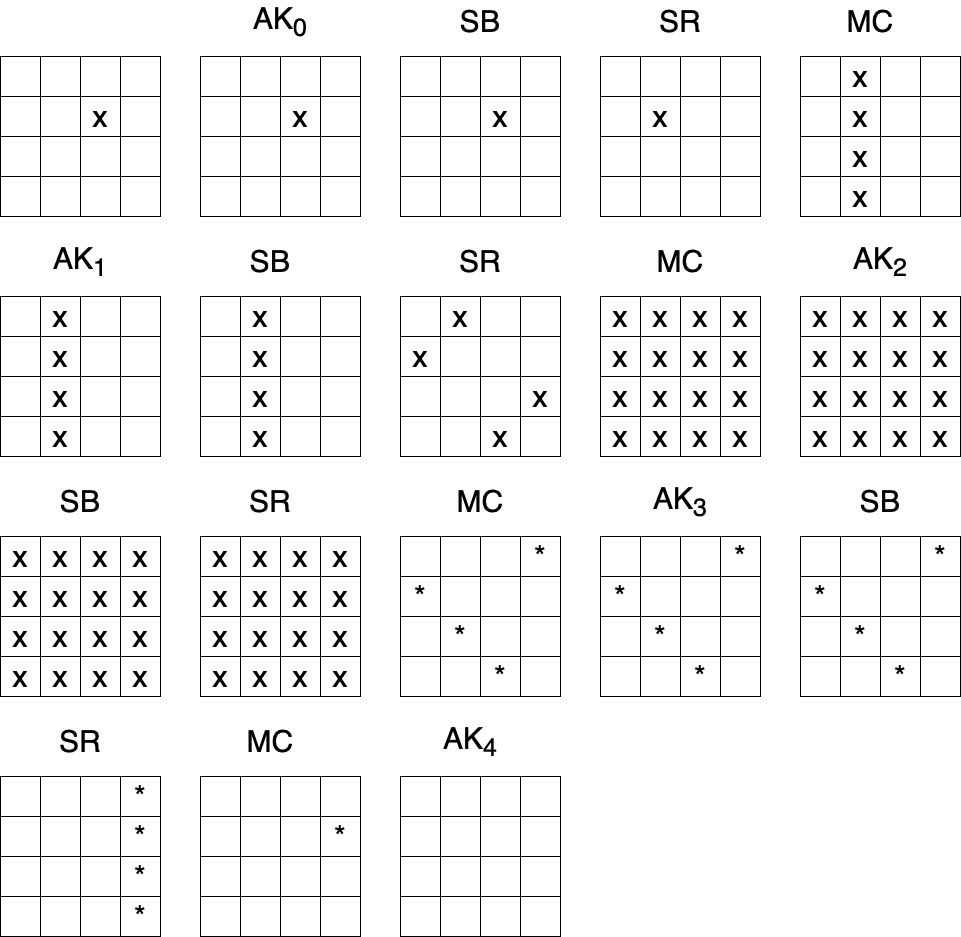
\includegraphics[scale=0.3]{aes-mc.png}
    \caption{Non-zero byte propagation example through AES. $AK_i$ denotes \texttt{AddRoundKey} of round $i$, $SB$ denotes \texttt{SubBytes}, $SR$ denotes \texttt{ShiftRows} and $MC$ denotes \texttt{MixColumns}. Note that the non-zero byte could be located anywhere, and the minimum number of active $S$-Boxes after 4 iterations would still be 25.}
    \label{fig:aes-trail}
\end{figure}

\bibliographystyle{plain}
\bibliography{refs}

\end{document}
